\section{有符号测度}
\label{sec:meas-signed}

测度只取非负值。可是很多量天然有正有负：一根杆上同时分布着正电荷与负电荷，一笔账在不同科目上有收入也有支出，两个概率分布在各个集合上的差有时为正、有时为负。最直接的模型是两个测度之差$\eta(A)=\nu(A)-\mu(A)$。本节研究这类赋值：它在哪里取正、在哪里取负，能否唯一地写回两个测度之差，以及怎样度量正负两方面的总量。积分尚未定义，本节只在集合层面讨论。

\subsection{正集与负集}
\label{sec:meas-positive-negative-sets}

\paragraph{从测度之差到有符号测度}
设$\nu,\mu$是$(X,\mathcal A)$上的测度，$\mu$有限。对两两不交的可测集$A_1,A_2,\dots$，两个测度各自可数可加，并且$\sum_n\mu(A_n)$收敛到有限值，所以
\[
 \eta\Bigl(\bigcup_nA_n\Bigr)=\sum_n\nu(A_n)-\sum_n\mu(A_n)=\sum_n\bigl(\nu(A_n)-\mu(A_n)\bigr)=\sum_n\eta(A_n).
\]
中间一步把两个级数逐项相减，这在至少一个级数有限时成立。可见$\eta=\nu-\mu$保留了可数可加性，只是不再非负；它可以取$+\infty$，但不会取$-\infty$。

两个无限测度不能直接相减。在$\mathbb N$上取计数测度$\nu$与$\mu=2\nu$，对无限集$A$，$\nu(A)-\mu(A)=+\infty-(+\infty)$没有定义。即使把它理解为某个数，也会和可数可加性冲突：$\mathbb N$分成单点后每块的差都是$-1$，级数和为$-\infty$；分成偶数集与奇数集后两块的差都没有定义。所以有符号测度必须禁止同时出现两种无穷。

\begin{definition}[有符号测度]
\label{def:meas-signed}
可测空间$(X,\mathcal A)$上的\term{有符号测度}（signed measure）是映射$\eta:\mathcal A\to[-\infty,+\infty]$，满足：$\eta$至多取$+\infty$与$-\infty$中的一个；$\eta(\varnothing)=0$；对任意两两不交的$A_1,A_2,\dots\in\mathcal A$，
\[
 \eta\Bigl(\bigcup_{n\geq1}A_n\Bigr)=\sum_{n\geq1}\eta(A_n),
\]
其中左端有限时，右端级数绝对收敛。若$\eta$只取有限实数值，称为\term{有限有符号测度}（finite signed measure）。
\end{definition}

“至多取一种无穷”保证了右端级数总有意义：各项中不会同时出现$+\infty$与$-\infty$。要求左端有限时级数绝对收敛，是因为不交集合的并与排列次序无关，右端也必须与次序无关；按实数级数的重排定理，这等价于绝对收敛。测度是有符号测度的特例，任意有限测度之差是有限有符号测度。

有符号测度是给\emph{集合}赋予实数的规则，不要与某些\emph{点}上取负值的函数混淆。$\eta(A)<0$表示集合$A$上的负质量多于正质量，这个数由整个集合决定。

\begin{example}[正负抵消]
\label{ex:meas-signed-weights}
取$X=\{1,2,3,4\}$及全部子集，规定单点值$\eta(\{1\})=2$，$\eta(\{2\})=-1$，$\eta(\{3\})=1$，$\eta(\{4\})=-2$，并令$\eta(A)=\sum_{i\in A}\eta(\{i\})$。它是有限有符号测度，也可以写成$\nu-\mu$，其中$\nu=2\delta_1+\delta_3$，$\mu=\delta_2+2\delta_4$。

计算几个值：$\eta(X)=2-1+1-2=0$，$\eta(\{1,2\})=1$，$\eta(\{1,3\})=3$，$\eta(\{2,4\})=-3$。全空间上的值为零只是正负抵消的结果；在$\{1,3\}$与$\{2,4\}$上，$\eta$的绝对值都达到$3$。所以$\eta(X)$很小甚至为零，不能说明$\eta$在各处都小。
\end{example}

例中的$\eta$还可以写成$(\nu+\delta_1)-(\mu+\delta_1)$。同一个有符号测度有许多种“测度减测度”的表示。我们要找的是由$\eta$本身确定、没有多余抵消的一种，第一步是找出$\eta$在哪里取正、在哪里取负。

\paragraph{正集与负集的定义}
只看$\eta(P)\geq0$并不够：例~\ref{ex:meas-signed-weights}中$\eta(\{1,2\})=1\geq0$，它的子集$\{2\}$却取$-1$。$\{1,2\}$整体为正，内部仍藏着负质量。要作为“正区域”，集合的每个可测部分都必须非负。

\begin{definition}[正集与负集]
\label{def:meas-positive-set}
设$\eta$是$(X,\mathcal A)$上的有符号测度。若$P\in\mathcal A$的每个可测子集$E$都满足$\eta(E)\geq0$，称$P$为$\eta$的\term{正集}（positive set）；若$N\in\mathcal A$的每个可测子集$E$都满足$\eta(E)\leq0$，称$N$为$\eta$的\term{负集}（negative set）。
\end{definition}

在例~\ref{ex:meas-signed-weights}中，$\{1,3\}$是正集，$\{2,4\}$是负集，$\{1,2\}$两者都不是。正集与负集可以同时是二者：$\eta$在其每个可测子集上都取零的集合，既是正集又是负集。

正集的可测子集仍是正集，可数个正集的并也是正集。若$P_1,P_2,\dots$是正集，$E\subseteq\bigcup_nP_n$可测，令$E_1=E\cap P_1$，$E_n=(E\cap P_n)\setminus(P_1\cup\dots\cup P_{n-1})$，则$E_n$是$P_n$的可测子集且两两不交，$\eta(E)=\sum_n\eta(E_n)\geq0$。负集同理。这两条封闭性是下面把正负区域拼起来的依据。

\subsection{Hahn分解与Jordan分解}
\label{sec:meas-hahn-jordan}

例~\ref{ex:meas-signed-weights}中，只要把$X$分成$\{1,3\}$与$\{2,4\}$，$\eta$在前一部分的每个子集上非负，在后一部分的每个子集上非正。一般的有符号测度是否也能一刀切成正、负两个区域？先对有限有符号测度证明，再说明扩展值的情形。

\paragraph{两条准备性质}
构造正负区域的思路是寻找使$\eta$最小的可测集。为此先要知道$\eta$的取值不会无限地向下延伸，并且单调集合列的连续性在有符号情形仍然成立。

\begin{lemma}[有限有符号测度有界]
\label{lem:meas-signed-bounded}
有限有符号测度$\eta$有界：存在$M<\infty$，使$\lvert\eta(A)\rvert\leq M$对一切$A\in\mathcal A$成立。
\end{lemma}

\begin{proof}
称可测集$A$是\emph{无界的}，如果$\sup\{\lvert\eta(E)\rvert:E\subseteq A,\ E\in\mathcal A\}=\infty$。设$X$是无界的，我们构造两两不交的可测集$B_1,B_2,\dots$，使每个$\lvert\eta(B_n)\rvert\geq1$。

设$A$无界。取可测子集$E\subseteq A$使$\lvert\eta(E)\rvert\geq\lvert\eta(A)\rvert+1$，则$\lvert\eta(A\setminus E)\rvert\geq\lvert\eta(E)\rvert-\lvert\eta(A)\rvert\geq1$。$E$与$A\setminus E$中至少有一个无界：否则$A$的任一可测子集$F$满足$\lvert\eta(F)\rvert\leq\lvert\eta(F\cap E)\rvert+\lvert\eta(F\setminus E)\rvert$，右边两项都有界。把无界的一块记为$A'$，另一块记为$B$，则$B\subseteq A\setminus A'$且$\lvert\eta(B)\rvert\geq1$。

从$A_0=X$出发反复执行这一步，得到无界集$A_0\supseteq A_1\supseteq\cdots$及$B_n\subseteq A_{n-1}\setminus A_n$，这些$B_n$两两不交。按定义~\ref{def:meas-signed}，$\sum_n\eta(B_n)$收敛到有限值$\eta(\bigcup_nB_n)$，通项必须趋于零，与$\lvert\eta(B_n)\rvert\geq1$矛盾。
\end{proof}

\begin{lemma}[有符号测度的单调连续性]
\label{lem:meas-signed-continuity}
设$\eta$是有限有符号测度。若$A_1\subseteq A_2\subseteq\cdots$，则$\eta(\bigcup_nA_n)=\lim_n\eta(A_n)$；若$A_1\supseteq A_2\supseteq\cdots$，则$\eta(\bigcap_nA_n)=\lim_n\eta(A_n)$。
\end{lemma}

\begin{proof}
对递增集合列，令$D_1=A_1$，$D_n=A_n\setminus A_{n-1}$，它们两两不交，$\bigcup_nA_n=\bigcup_nD_n$，部分和$\sum_{k\leq n}\eta(D_k)=\eta(A_n)$，由可数可加性得结论。对递减集合列，$A_1\setminus A_n$递增，并为$A_1\setminus\bigcap_nA_n$；由已证部分及$\eta(A_1\setminus B)=\eta(A_1)-\eta(B)$（各项有限），得$\eta(A_1)-\eta(\bigcap_nA_n)=\lim_n(\eta(A_1)-\eta(A_n))$。
\end{proof}

与测度不同，这里递减情形不需要另加有限性假设，因为$\eta$本身只取有限值。

\paragraph{Hahn分解}
若某个可测集$D$使$\eta$达到最小值，那么从$D$中拿走一个正值子集，或向$D$中添入一个负值的外部集合，都会让取值更小，这不可能；于是$D$是负集，补集是正集。难点在于证明最小值确实能被某个集合达到。

\begin{theorem}[Hahn分解]
\label{thm:meas-hahn}
设$\eta$是$(X,\mathcal A)$上的有符号测度。则存在$P\in\mathcal A$，使$P$是$\eta$的正集，$N=X\setminus P$是$\eta$的负集。这样的一对$(P,N)$称为$\eta$的\term{Hahn分解}（Hahn decomposition）。若$(P',N')$是另一组Hahn分解，则$P\cap N'$与$P'\cap N$的每个可测子集上$\eta$都取零。
\end{theorem}

\begin{proof}
先设$\eta$有限。令$m=\inf_{A\in\mathcal A}\eta(A)$。由引理~\ref{lem:meas-signed-bounded}，$m$是有限实数，又$\eta(\varnothing)=0$，故$m\leq0$。对每个$n$取可测集$A_n$使$\eta(A_n)<m+2^{-n}$。

第一步说明两个近乎最小的集合取交后仍近乎最小。对可测集$A,B$，有限可加性给出$\eta(A\cup B)+\eta(A\cap B)=\eta(A)+\eta(B)$；又$\eta(A\cup B)\geq m$，所以$\eta(A\cap B)\leq\eta(A)+\eta(B)-m$。固定$n$，对$k\geq n$令$C_{n,k}=A_n\cap\dots\cap A_k$，对$k$归纳得
\[
 \eta(C_{n,k+1})\leq\eta(C_{n,k})+\eta(A_{k+1})-m<m+\sum_{j=n}^{k+1}2^{-j}<m+2^{1-n}.
\]

第二步取极限。$C_{n,k}$关于$k$递减，令$C_n=\bigcap_{k\geq n}A_k$；由引理~\ref{lem:meas-signed-continuity}，$\eta(C_n)\leq m+2^{1-n}$。$C_n$关于$n$递增，令$D=\bigcup_nC_n$；再由该引理，$\eta(D)=\lim_n\eta(C_n)\leq m$。另一方面$\eta(D)\geq m$，所以$\eta(D)=m$，最小值被$D$达到。

第三步验证符号。若可测集$E\subseteq D$满足$\eta(E)>0$，则$\eta(D\setminus E)=m-\eta(E)<m$，矛盾，所以$D$是负集。若可测集$E\subseteq X\setminus D$满足$\eta(E)<0$，则$\eta(D\cup E)=m+\eta(E)<m$，同样矛盾，所以$X\setminus D$是正集。取$N=D$，$P=X\setminus D$即可。

对允许取一种无穷值的$\eta$，存在性的证明需要另一条引理：有限正值的集合中总能找到正值的正集。由此可以在正集中取使$\eta$接近上确界的一列，再用正集的可数并封闭性拼成最大的正区域。这里不给出这部分证明，可参考Folland的《Real Analysis》第3章。

最后看两组分解的差别，这一步对两种情形都适用。$P\cap N'$既是正集$P$的子集，又是负集$N'$的子集，它的每个可测子集$E$同时满足$\eta(E)\geq0$与$\eta(E)\leq0$，即$\eta(E)=0$。$P'\cap N$同理。
\end{proof}

Hahn分解一般不唯一：$\eta$在其上完全为零的区域可以划给任意一侧。在实轴上令$\eta=\lambda|_{[0,1]}-\lambda|_{[2,3]}$，$P_1=(-\infty,3/2)$与$P_2=(-\infty,2)$都给出Hahn分解，两者相差的$[3/2,2)$上$\eta$的每个子集都取零，见图~\ref{fig:meas-hahn-decomposition}。正区域还可以只差一个Lebesgue零测集，例如把点$1/2$从$P_1$移到负区域一侧。

\begin{figure}[!htbp]
  \centering
  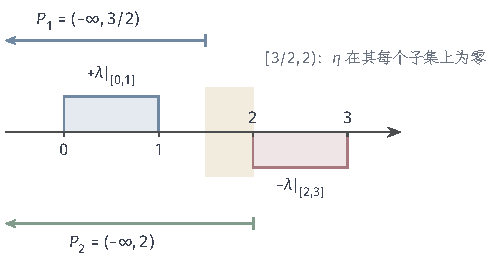
\includegraphics[width=84.06mm]{figures/02-abstract-mathematics/01-metric-and-measure/tikz/c2-hahn-decomposition/figure.pdf}
  \caption{Hahn分解的区域选择不唯一。$\eta=\lambda|_{[0,1]}-\lambda|_{[2,3]}$，蓝块在$[0,1]$上表示正的长度，红块在$[2,3]$上表示负的长度，块高表示长度测度前的系数$\pm1$。正区域可以取$P_1=(-\infty,3/2)$，也可以取$P_2=(-\infty,2)$；二者之差$[3/2,2)$（黄色）的每个可测子集上$\eta$都为零，所以放在哪一侧都不改变符号要求。}
  \label{fig:meas-hahn-decomposition}
\end{figure}

\paragraph{Jordan分解}
区域可以不同，限制在区域上的质量却是唯一的。把$\eta$分别限制到正区域与负区域，就得到两个测度。

\begin{theorem}[Jordan分解]
\label{thm:meas-jordan}
设$\eta$是有符号测度，$(P,N)$是它的一组Hahn分解。令
\[
 \eta^+(A)=\eta(A\cap P),\qquad \eta^-(A)=-\eta(A\cap N),\qquad A\in\mathcal A .
\]
则$\eta^+,\eta^-$是测度，其中至少一个有限，$\eta=\eta^+-\eta^-$，且$\eta^+(N)=\eta^-(P)=0$；它们不依赖于Hahn分解的选取。反过来，若$\eta=\alpha-\beta$，其中$\alpha,\beta$是测度、至少一个有限，并且存在可测集$S$使$\beta(S)=0$、$\alpha(X\setminus S)=0$，则$\alpha=\eta^+$，$\beta=\eta^-$。这个表示称为$\eta$的\term{Jordan分解}（Jordan decomposition），$\eta^+$、$\eta^-$分别称为$\eta$的\term{正变差}（positive variation）与\term{负变差}（negative variation）。
\end{theorem}

\begin{proof}
$A\cap P$是正集的子集，所以$\eta^+(A)\geq0$；同理$\eta^-(A)\geq0$。可数可加性直接来自$\eta$：若$A_n$两两不交，则$A_n\cap P$也两两不交。若$\eta$不取$+\infty$，则$\eta^+(X)=\eta(P)<+\infty$；若不取$-\infty$，则$\eta^-$有限。由$A=(A\cap P)\cup(A\cap N)$得$\eta(A)=\eta^+(A)-\eta^-(A)$，右边至多一项无穷，所以差有意义。$\eta^+(N)=\eta(\varnothing)=0$，$\eta^-(P)=0$。

再看与Hahn分解无关。设$(P',N')$是另一组分解。由定理~\ref{thm:meas-hahn}，$A\cap P\cap N'$与$A\cap P'\cap N$上$\eta$取零，因此
\[
 \eta(A\cap P)=\eta(A\cap P\cap P')+\eta(A\cap P\cap N')=\eta(A\cap P\cap P')=\eta(A\cap P'),
\]
最后一步对$P'$作同样的拆分。$\eta^-$同理。

最后证唯一性。设$\eta=\alpha-\beta$与$S$如定理所述。对$S$的可测子集$E$，$\eta(E)=\alpha(E)-0\geq0$；对$X\setminus S$的可测子集$E$，$\eta(E)=0-\beta(E)\leq0$。所以$(S,X\setminus S)$本身是一组Hahn分解。由已证的无关性，$\eta^+(A)=\eta(A\cap S)=\alpha(A\cap S)=\alpha(A)$，最后一步用了$\alpha(A\setminus S)=0$。同理$\beta=\eta^-$。
\end{proof}

定理中“存在$S$使$\beta(S)=0$、$\alpha(X\setminus S)=0$”说的是两个测度分别集中在两个不交的集合上，这种关系称为相互奇异，第~\ref{chap:measure-densities}章再系统比较。唯一性离不开这一条件。仍取$\eta=\lambda|_{[0,1]}-\lambda|_{[2,3]}$，它的Jordan分解是$\eta^+=\lambda|_{[0,1]}$、$\eta^-=\lambda|_{[2,3]}$。另一方面，令$\alpha=\lambda|_{[0,3]}$，$\beta=\lambda|_{[1,2]}+2\lambda|_{[2,3]}$，逐段检查系数：$[0,1]$上为$1-0$，$[1,2]$上为$1-1$，$[2,3]$上为$1-2$，所以同样有$\alpha-\beta=\eta$。但$\alpha,\beta$在$[1,3]$上重叠，总量都是$3$，而$\eta^\pm$的总量都是$1$。

这种多余的重叠只增不减。对任意表示$\eta=\alpha-\beta$（$\alpha,\beta$为测度，至少一个有限）及任意$A\in\mathcal A$，
\[
 \eta^+(A)=\eta(A\cap P)=\alpha(A\cap P)-\beta(A\cap P)\leq\alpha(A\cap P)\leq\alpha(A),
\]
同理$\eta^-(A)\leq\beta(A)$。所以Jordan分解是所有“测度减测度”表示中最小的一个。两种分解的输出不同：Hahn分解输出一个集合划分，它不唯一；Jordan分解输出两个测度，它唯一。

\subsection{全变差}
\label{sec:meas-total-variation}

$\lvert\eta(A)\rvert$衡量的是集合$A$上正负相抵后的净值，例~\ref{ex:meas-signed-weights}说明它可能掩盖很大的局部差别。要累计正负两方面的全部质量，应当把正变差与负变差相加，而不是相减。

\begin{definition}[全变差]
\label{def:meas-total-variation}
设$\eta$是有符号测度，$\eta=\eta^+-\eta^-$是它的Jordan分解。称测度
\[
 \lvert\eta\rvert=\eta^++\eta^-
\]
为$\eta$的\term{全变差测度}（total variation measure），称$\lvert\eta\rvert(X)$为$\eta$的\term{全变差}（total variation）。
\end{definition}

\paragraph{分割刻画}
$\lvert\eta\rvert$也可以不借助Jordan分解，直接从$\eta$的取值读出：把$A$切成有限块，对每块的净值取绝对值再相加。切得越合适，抵消越少；最合适的切法就是沿Hahn分解切开。

\begin{theorem}[全变差的分割刻画]
\label{thm:meas-total-variation-partition}
对每个$A\in\mathcal A$，
\[
 \lvert\eta\rvert(A)=\sup\Bigl\{\sum_{i=1}^k\lvert\eta(A_i)\rvert:\ k\geq1,\ A_1,\dots,A_k\in\mathcal A\text{两两不交},\ \bigcup_{i=1}^kA_i=A\Bigr\}.
\]
\end{theorem}

\begin{proof}
对$A$的任一有限可测分割，
\[
 \sum_i\lvert\eta(A_i)\rvert=\sum_i\lvert\eta^+(A_i)-\eta^-(A_i)\rvert\leq\sum_i\bigl(\eta^+(A_i)+\eta^-(A_i)\bigr)=\lvert\eta\rvert(A),
\]
所以上确界不超过$\lvert\eta\rvert(A)$。取Hahn分解$(P,N)$及分割$A_1=A\cap P$、$A_2=A\cap N$，则$\lvert\eta(A_1)\rvert+\lvert\eta(A_2)\rvert=\eta^+(A)+\eta^-(A)=\lvert\eta\rvert(A)$，上确界被达到。
\end{proof}

回到例~\ref{ex:meas-signed-weights}。不分割时$\lvert\eta(X)\rvert=0$；分成$\{1,2\}$与$\{3,4\}$时得$\lvert1\rvert+\lvert-1\rvert=2$；分成$\{1,3\}$与$\{2,4\}$时得$3+3=6$。再细分也不会超过$6$，因为四个单点上的绝对值之和为$2+1+1+2=6$。所以$\lvert\eta\rvert(X)=6$，正好由正负区域的分割取得，见图~\ref{fig:meas-total-variation-partition}。

\begin{figure}[!htbp]
  \centering
  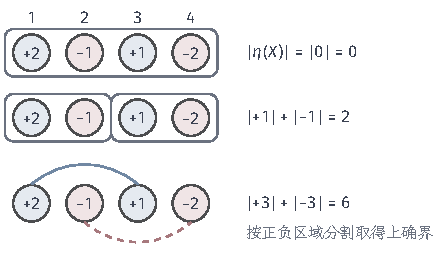
\includegraphics[width=75.128mm]{figures/02-abstract-mathematics/01-metric-and-measure/tikz/c2-total-variation-partition/figure.pdf}
  \caption{用分割读取全变差。四个点的权重为$+2,-1,+1,-2$。第一行不分割，净值为$0$；第二行把相邻的正负点合在一起，仍有抵消，绝对值之和为$2$；第三行按符号分组（蓝色实弧连接正点，红色虚弧连接负点），没有抵消，绝对值之和为$6=\lvert\eta\rvert(X)$。}
  \label{fig:meas-total-variation-partition}
\end{figure}

\paragraph{净值与总量}
由分割刻画取平凡分割$\{A\}$，立即得到$\lvert\eta(A)\rvert\leq\lvert\eta\rvert(A)$：左边允许抵消，右边累计正负变化的总量。特别地，$\lvert\eta\rvert(A)=0$当且仅当$\eta$在$A$的每个可测子集上都取零。所以$\lvert\eta\rvert$的零测集正是$\eta$完全看不见的集合；对有符号测度说“几乎处处”时，都相对于$\lvert\eta\rvert$来理解。

\paragraph{有限与扩展值两种情形}
若$\eta$是有限有符号测度，$\eta^+$与$\eta^-$都有限，$\lvert\eta\rvert$是有限测度，并且$\lvert\eta(A)\rvert\leq\lvert\eta\rvert(X)<\infty$对一切$A$成立，这与引理~\ref{lem:meas-signed-bounded}一致。若$\eta$取$+\infty$，则$\eta^+$无限而$\eta^-$有限，$\lvert\eta\rvert$在某些集合上为$+\infty$，此时只能在$\lvert\eta\rvert$有限的集合上作数值比较。

两个概率测度$P,Q$之差$\eta=P-Q$属于前一种情形。由$\eta(X)=0$得$\eta^+(X)=\eta^-(X)=\tfrac12\lvert\eta\rvert(X)$。又对每个可测集$A$有$\eta(A)\leq\eta^+(A)\leq\eta^+(X)$，取$A=P$时等号成立，所以
\[
 \tfrac12\lvert P-Q\rvert(X)=\eta^+(X)=\sup_{A\in\mathcal A}\bigl(P(A)-Q(A)\bigr).
\]
后续估计积分误差时，常用总量有限的$\lvert\eta\rvert$控制正负两方面的贡献；一个有符号测度何时能写成某个可积函数乘以参考测度，留到第~\ref{chap:measure-densities}章，那里同样要区分总量有限与允许扩展值的情形。
